\subsection{Background: Bilateral Filtering and the Bilateral Grid}

\label{sec:hfbs-background}

We base our design for fast and accurate VR video on a state-of-the-art bilateral-space optimization algorithm, the bilateral solver~\cite{BarronPoole2016}. 
The bilateral solver is general-purpose and scalable, and can be applied to the many vision applications: optical flow, stereo, depth superresolution, image colorization, and semantic segmentation.
The bilateral solver can be used as part of an edge-aware optical flow algorithm for VR video, and scales to high resolutions efficiently \cite{googlejump}.

  \begin{figure}[h]
		\centering
		\includegraphics[width=\columnwidth]{hfbs-figs/depth_estimation_steps.pdf}
		\caption{Our bilateral solver produces smooth, edge-aware flow fields.  Given an input pair of images (a), a low-resolution flow is estimated (b),  upsampled to a noisy high-resolution flow (c), and processed with the bilateral solver (d)  to produce an edge-aware smoothed flow (e). Our algorithm for bilateral solving is better-suited for hardware acceleration and results in speedups of up to 50$\times$ over prior work \cite{googlejump, BarronPoole2016}.}
		\label{fig:teaser}
  \end{figure}

This optical flow algorithm generates a correspondence map from a pair of images by computing a rough flow vector for every pixel (Figure~\ref{fig:teaser}b-c), and then refining that flow field until a cost function has been minimized. 
To compute this edge-aware per-pixel flow field, the bilateral solver resamples a coarse flow field into \emph{bilateral-space} (Figure~\ref{fig:teaser}d), and then solves an optimization problem in bilateral-space to infer the smoothest possible flow-field that is similar to the input coarse flow field. 
In bilateral-space, simple local filters are equivalent to costly, global, edge-aware filters in pixel-space---consequently, flow refinement in bilateral-space is much faster than its pixel-space equivalent.
We perform optimization in a three-dimensional \emph{bilateral grid} data structure \cite{Chen2007}. 

Figure~\ref{fig:teaser} describes how we map our optical flow problem to the bilateral solver. We first compute a coarse, tile-based flow field, shown in Figure~\ref{fig:teaser}b, and then upsample it to noisy flow field. As seen in the figure, the upsampled flow in Figure~\ref{fig:teaser}c is very noisy, so we use the bilateral solver to smooth our noisy flow field while maintaining information . This last step (shown as a dotted box in Figure~\ref{fig:teaser}) translates into a computation-intensive optimization problem since multiple factors must be considered. 

To solve the optimization problem, the bilateral solver resamples the problem into \emph{bilateral space}, which is a multi-dimensional space that allows edge-aware operations to be performed on an image.
Figure ~\ref{fig:bilateral_grid_3d} illustrates a simplified version of bilateral space and its use in our problem.
We begin with the noisy flow field of Figure~\ref{fig:bilateral_grid_3d}a-i, where color corresponds to some flow value. 
If we attempt to denoise this noisy flow field by applying a simple smoothing kernel, the result will present undesirable blurring at color edges. 
In Figure~\ref{fig:bilateral_grid_3d}a-ii, for instance, the green region is successfully denoised, but the blue and red regions (which likely belong to different objects) blend around the edges, producing incorrect flow values there.

\begin{figure*}[h]
  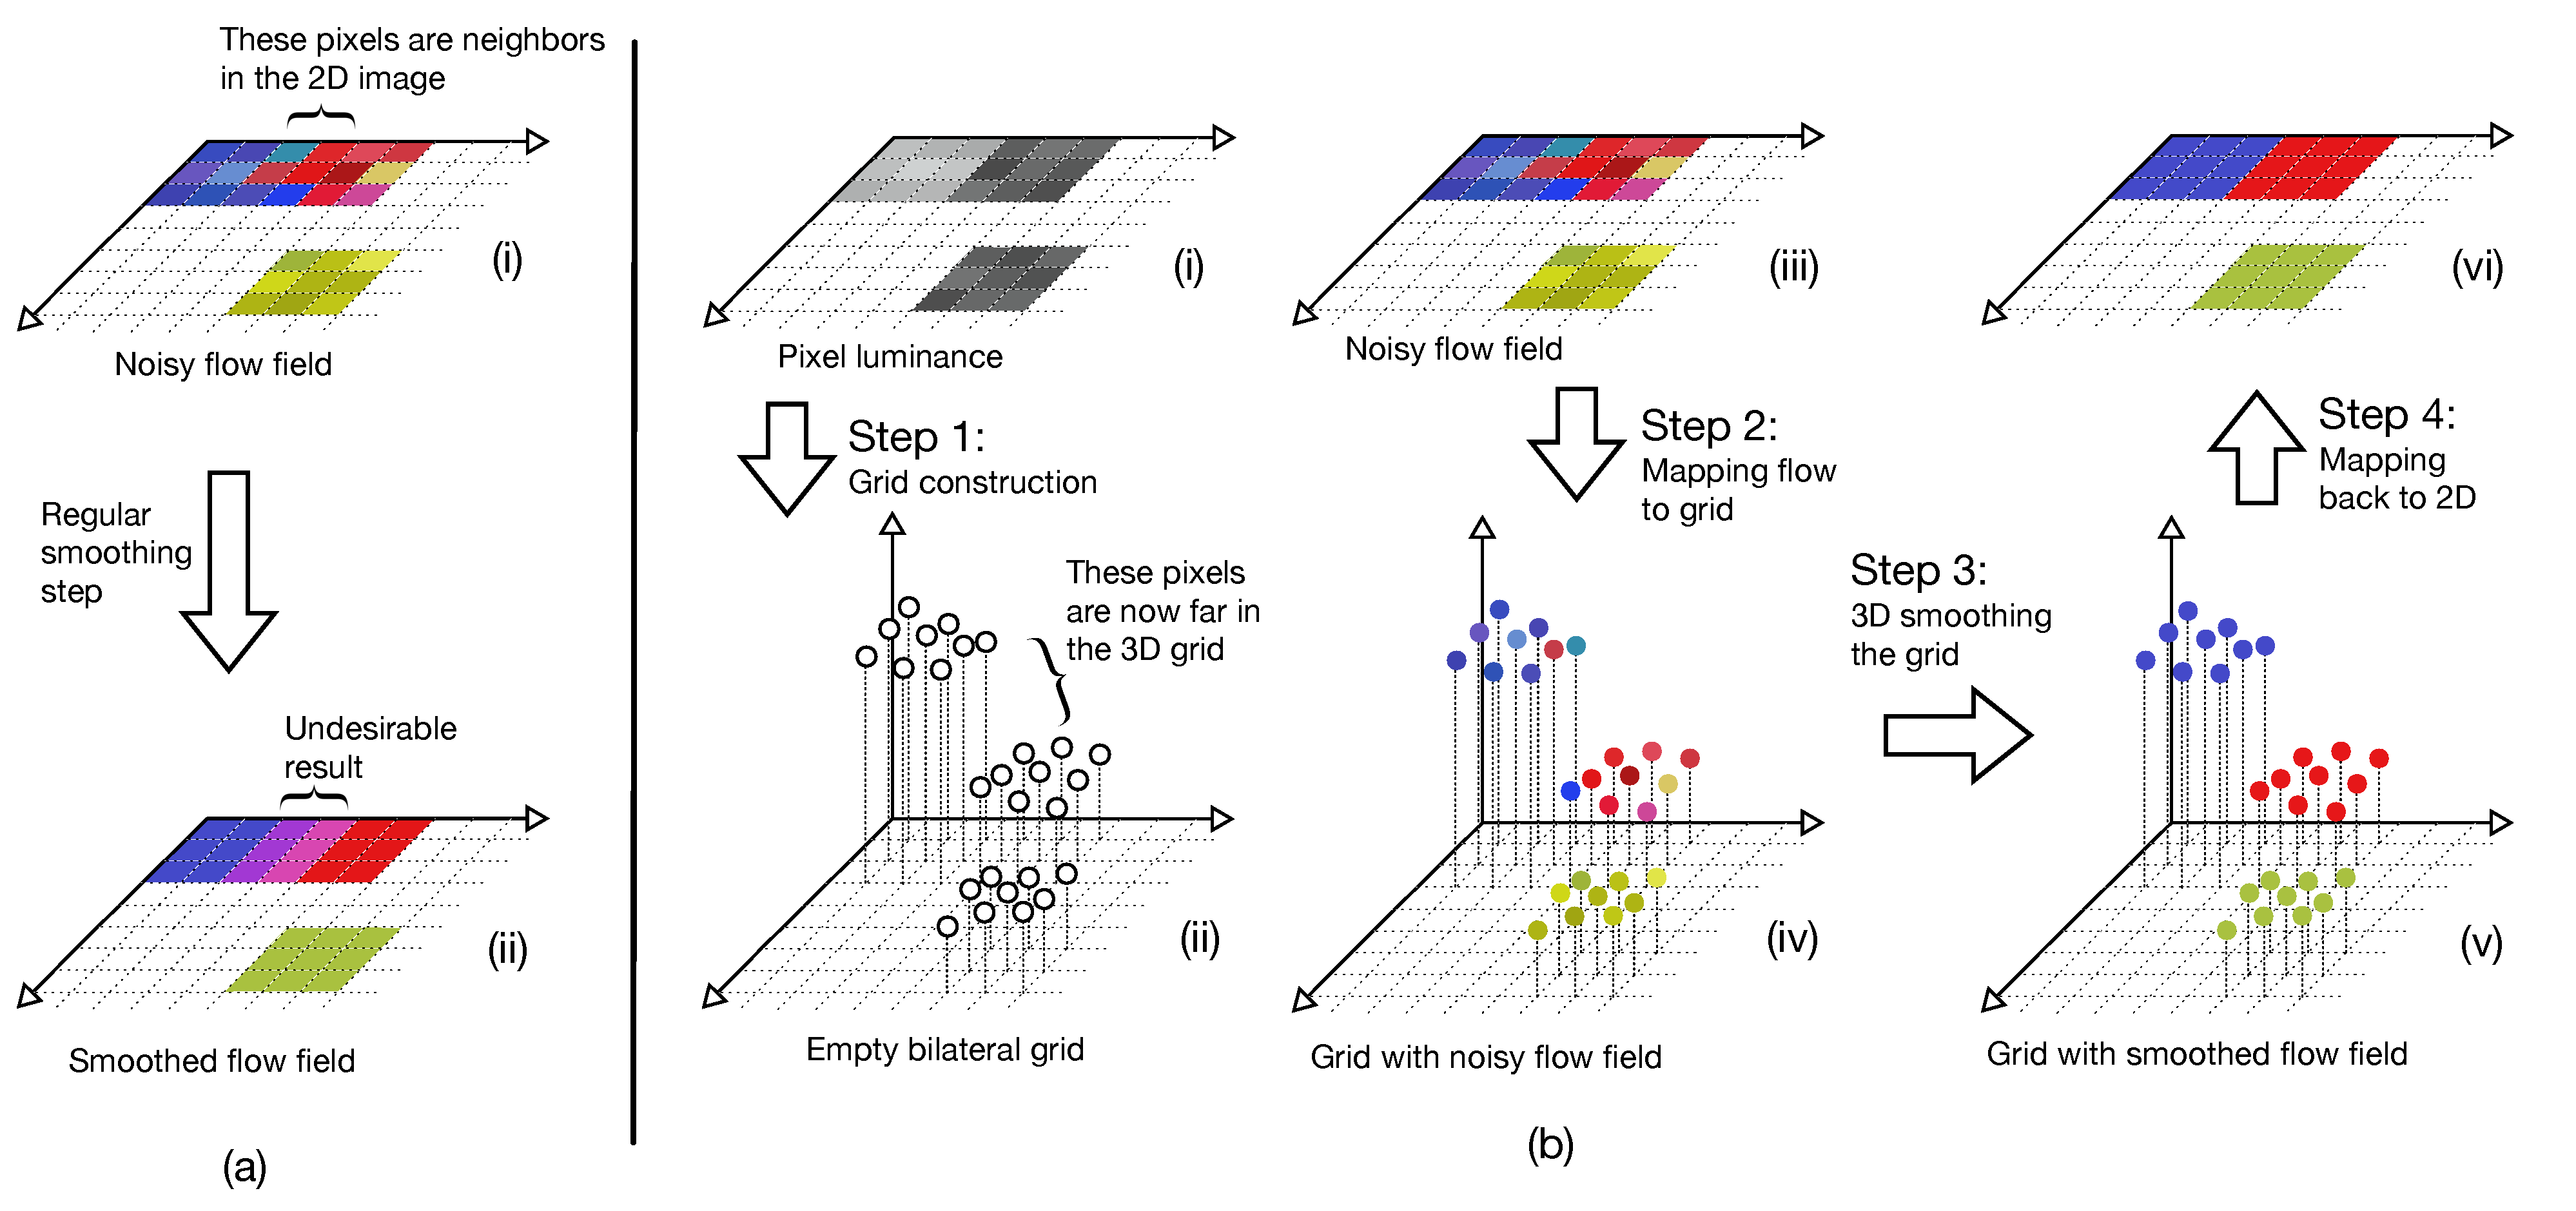
\includegraphics[width=.9\textwidth]{hfbs-figs/bilateral_grid_3d.pdf}
  \caption{Smoothing a noisy flow field in (a) regular 2D space and (b) bilateral space. Regular smoothing produces undesirable artifacts at edges as the flow values blur together. The bilateral grid allows edge-aware smoothing and produces a correct denoised output.}
  \label{fig:bilateral_grid_3d}
\end{figure*}


To smooth this flow field while maintaining sharp edges, we map the problem to bilateral space. 
First, we construct a \emph{bilateral grid} for the original image, where a pixel in the image at location $(x,y)$ with luminance $l$ corresponds to a grid block at location $(x,y,l)$ (Figure~\ref{fig:bilateral_grid_3d}b-i, b-ii). 
In the 3D bilateral space, the lighter pixels are separated from neighboring darker pixels. 
We then map the flow value of each pixel (Figure~\ref{fig:bilateral_grid_3d}b-iii) to its corresponding grid location (Figure~\ref{fig:bilateral_grid_3d}b-iv).
When we smooth this noisy flow in bilateral space, the blue and red areas are no longer neighbors and do not affect each other's value. 
Finally, we map the smoothed 3D flow (Figure~\ref{fig:bilateral_grid_3d}b-v) back to the 2D representation (Figure~\ref{fig:bilateral_grid_3d}b-vi). 
The resulting  bilateral-smooth output in Figure~\ref{fig:bilateral_grid_3d}a-vi retains sharp edges.



